Firebase es una plataforma propiedad de Google que tiene como objetivo proporcionar un enfoque holístico para un rápido desarrollo web y móvil. En resumen, le permite centrarse en las partes frontales de la aplicación. Se completa con una base de datos visual sin tablas (NoSQL), alojamiento, almacenamiento de archivos, procesamiento del lado del servidor para cosas que deben protegerse de la interfaz y un sistema de autenticación, todo lo necesario para aplicaciones pequeñas y medianas. \\[0.8cm]
% \subsection{Servicios de Firebase}
% \begin{itemize}
%   \item Base de datos
%   \item Autenticación
%   \item Almacenamiento
%   \item Notificaciones
%   \item Análisis
% \end{itemize}
Cloud Firestore es el servicio de base de datos de Google Firebase para aplicaciones móviles. Firestore permite una experiencia de programación increíble cuando se usa en un stack de aplicaciónes completo. Los datos en tiempo real y la facilidad de conexión a la base de datos hacen que la pila FERN sea una forma rápida de conectar estas tecnologías. 
\subsection{Componentes}
\begin{itemize}
  \item Firebase (base de datos)
  \item Express.js (servidor)
  \item React.js (cliente)
  \item Node.js (entorno del servidor)
\end{itemize}
\begin{figure}[H]
  \centering
  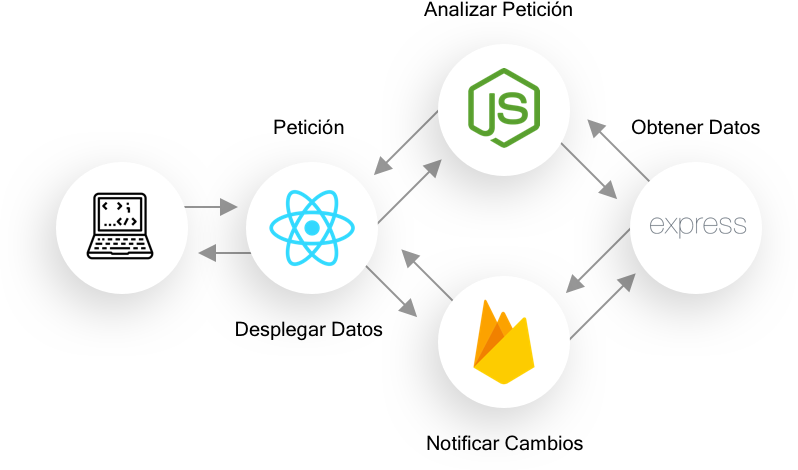
\includegraphics[width=0.8\textwidth]{fern}
  \caption{Flujo de informacion en FERN Stack.}
\end{figure}
\subsection{Cloud Firestore}
Firestore es una bases de datos orientada a documentos, toda la información se guarda en colecciones como JSON, principalmente diseñada para almacenar, recuperar y administrar información orientada a documentos, también conocida como datos semiestructurados.\\[0.8cm]
La escalabilidad es completamente automática, lo que significa que no es necesario compartir sus datos en varias instancias. Los cargos de Cloud Firestore se basan en las operaciones realizadas en su base de datos (lectura, escritura, borrado), ancho de banda y almacenamiento. Admite límites de gasto diario para proyectos de Google App Engine, para garantizar que no exceda los costos con los que el usuario se sienta cómodo.
\begin{figure}[H]
  \centering
  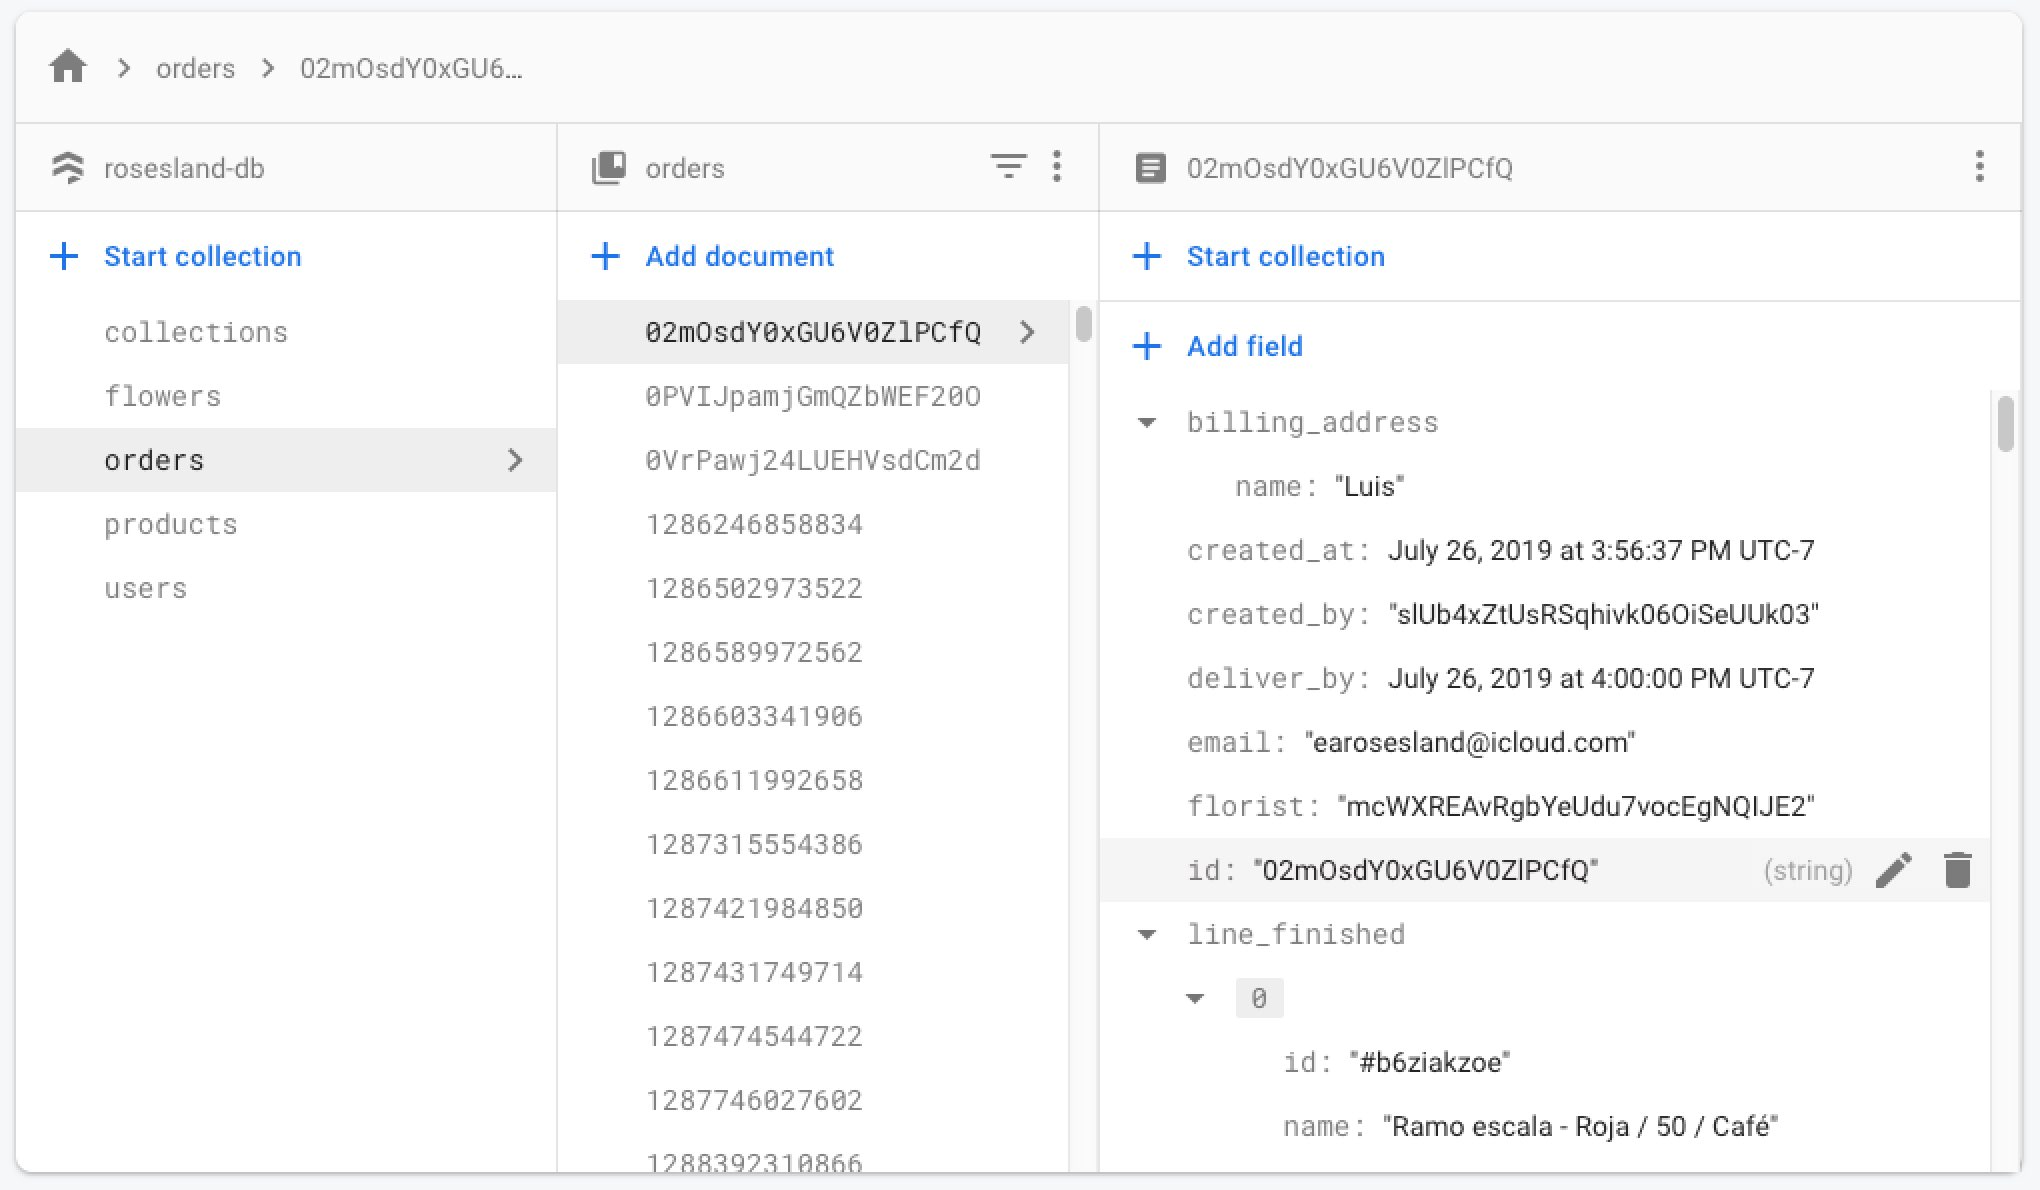
\includegraphics[width=0.9\textwidth]{firestore}
  \caption{Colección de Firestore con sus documentos internos.}
\end{figure}
\subsection{Node.js}
Node.js es un entorno multiplataforma de código abierto para ejecutar código JavaScript del lado del servidor. El entorno de tiempo de ejecución de Node.js incluye todo lo que necesita para ejecutar un programa escrito en JavaScript. \\[0.8cm]
Node.js surgió cuando los desarrolladores originales de JavaScript lo extendieron de algo que solo podía ejecutar en el navegador a algo que podría ejecutar en su máquina como una aplicación independiente. Ahora puede hacer mucho más con JavaScript que simplemente hacer que los sitios web sean interactivos. JavaScript ahora tiene la capacidad de hacer cosas que otros lenguajes de secuencias de comandos como Python pueden hacer. Tanto su navegador JavaScript como Node.js se ejecutan en el motor de tiempo de ejecución JavaScript V8. Este motor toma su código JavaScript y lo convierte en un código de máquina más rápido. El código de máquina es un código de bajo nivel que la computadora puede ejecutar sin necesidad de interpretarlo primero.
\begin{figure}[H]
  \centering
  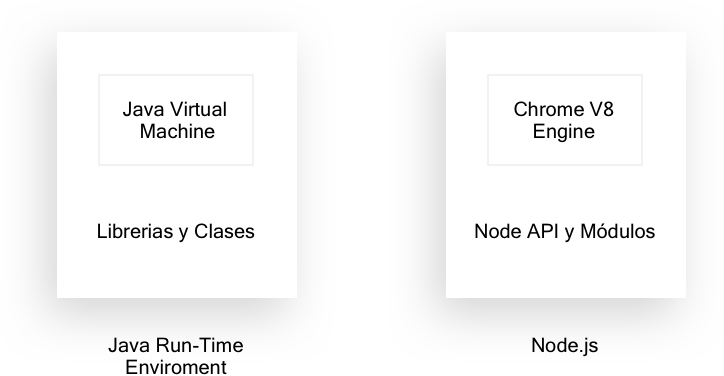
\includegraphics[width=0.8\textwidth]{node}
  \caption{Analogía Node.js con Java.}
\end{figure}
\subsubsection{Motor V8 de Google Chrome}
Node.js utiliza el motor de ejecución ultra rápido V8 de Google Chrome. Hasta el lanzamiento de Chrome, la mayoría de los navegadores leían JavaScript de manera ineficiente: el código se leía e interpretaba poco a poco. Tomó mucho tiempo leer JavaScript y convertirlo a lenguaje máquina para que el procesador pudiera entenderlo. \\[0.8cm]
El motor V8 de Google Chrome funciona completamente diferente. Está altamente optimizado y lleva a cabo lo que llamamos compilación JIT (Just In Time). Transforma rápidamente el código JavaScript en lenguaje máquina.
% \subsubsection{Características}
% \begin{itemize}
  %   \item Node.js utiliza un modelo de E/S (I/O) sin bloqueo controlado por eventos que lo hace ligero y eficiente.
  
  %   \item El ecosistema de paquetes de Node.js, \textit{npm}, es el ecosistema de bibliotecas de código abierto más grande del mundo.
% \end{itemize}
\subsection{El ecosistema NPM}
NPM (Node Package Manager) es el administrador de paquetes predeterminado para Node.js. se instala en el sistema con la instalación de Node.js. Los paquetes y módulos necesarios en un proyecto Node se instalan utilizando \textit{npm}.\\[0.8cm]
NPM consta de tres componentes:
\begin{enumerate}
  \item Sitio web
  \item Registro
  \item CLI
\end{enumerate}
\subsubsection{Sitio web}
El sitio web oficial de npm es https://www.npmjs.com/. Con este sitio web puede encontrar paquetes, ver documentación, compartir y publicar paquetes.
\subsubsection{Registro}
El registro npm es una gran base de datos que consta de más de medio millón de paquetes. Los desarrolladores descargan paquetes del registro npm y publican sus paquetes en el registro.
\subsubsection{CLI (interfaz de línea de comando)}
Esta es la línea de comando que ayuda a interactuar con el npm para instalar, actualizar y desinstalar paquetes y administrar dependencias.
\subsection{Comandos NPM}
Npm tiene muchos paquetes que puedes usar en una aplicación para que su desarrollo sea más rápido y eficiente. Instalar módulos usando NPM no representa un gran problema. Hay una sintaxis simple para instalar cualquier módulo Node.js:
\begin{verbatim}
  npm install <Nombre del módulo>
  ejemplo:
  npm install express
\end{verbatim}
\subsection{Express.js}
Escribir un servidor web completo a mano en Node.js directamente no es tan fácil, ni es necesario, Express.js es un paquete de aplicación web minimalista y extensible creado para el ecosistema Node.js. Permite crear un servidor web legible, flexible y fácil de mantener. \\[0.8cm]
Express.js le permite definir rutas, especificaciones de qué hacer cuando llega una solicitud HTTP que coincide con un patrón determinado. La especificación coincidente se basa en expresiones regulares (regex) y es muy flexible, como la mayoría de los otros entornos de aplicaciones web. La parte de qué hacer es solo una función que recibe la solicitud HTTP analizada. \\[0.8cm]
Express.js analiza la URL de solicitud, encabezados y parámetros. En el lado de la respuesta, tiene, como se esperaba, toda la funcionalidad requerida por las aplicaciones web. Esto incluye la configuración de códigos de respuesta, configuración de cookies, envío de encabezados personalizados, etc. Además, puede escribir middleware Express, piezas de código personalizadas que se pueden insertar en cualquier ruta de procesamiento de solicitud/respuesta para lograr una funcionalidad común como el registro, la autenticación, entre otras.
\subsection{React.js}
React es una biblioteca de JavaScript declarativa, eficiente y flexible creada en 2013 por el equipo de desarrollo de Facebook. React quería que las interfaces de usuario fueran más modulares (o reutilizables) y más fáciles de mantener. Según el sitio web de React, se utiliza para \textit{construir componentes encapsulados que administran su propio estado, y unirlos para crear interfaces de usuario complejas}. React es una biblioteca JavaScript que permite componer interfaces de usuario complejas a partir de piezas de código pequeñas y aisladas llamadas \textit{componentes}.
\subsection{Componentes}
Un componente es una pequeña parte de la interfaz de usuario. Todas las piezas reutilizables de una página web se abstraen en un componente.
\begin{figure}[H]
  \centering
  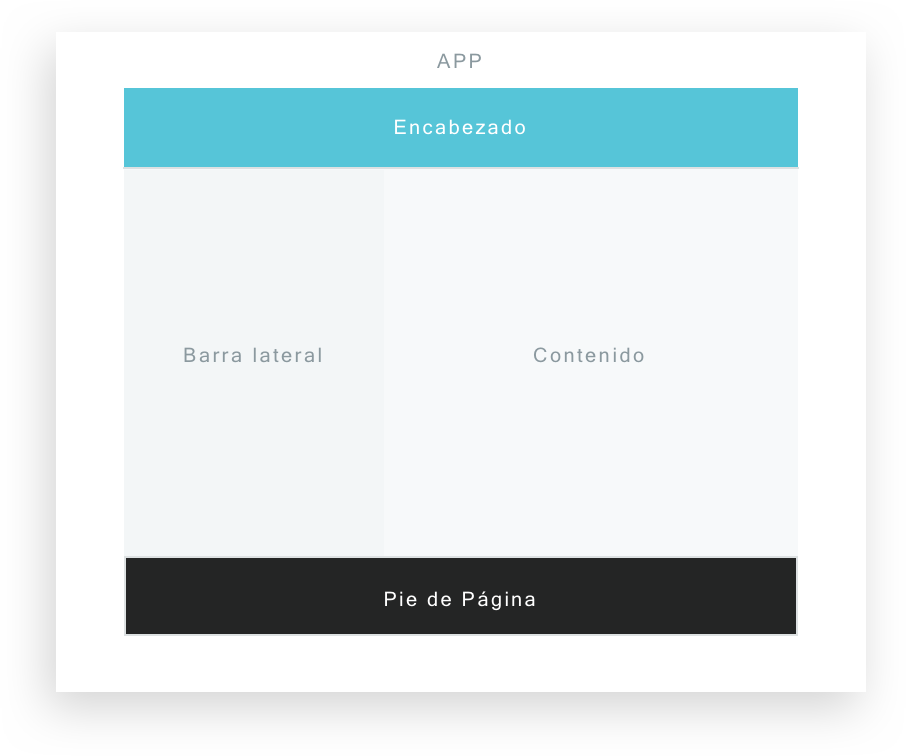
\includegraphics[width=0.8\textwidth]{components}
  \caption{Componentes principales de una página web.}
\end{figure}
En primer lugar, hay un componente principal llamado componente APP. Este componente de la aplicación contiene cuatro componentes secundarios o se divide en cuatro componentes:
\begin{enumerate}
  \item Encabezado
  \item Barra lateral
  \item Contenido
  \item Pie de página
\end{enumerate}
La función de cada componente se manejará independientemente con otros componentes. Cada componente es una pieza reutilizable, y se puede pensar en cada componente de forma aislada.